% figure_style.tex — Appendix: Figure Style Guide
\chapter{Figure Style Guide}

% Macro: compact margin figure with caption text
\newcommand{\marginfig}[2]{%
  \marginnote{\centering\includegraphics[width=1.15in]{#1}\par\footnotesize #2}%
}

This appendix defines conventions for figures, tables, and margin notes, ensuring typographic and visual consistency across the dissertation. 
It is inspired by Edward Tufte’s principles of data-ink maximization, small multiples, and sparklines.

\section{General Principles}
\begin{itemize}
  \item \textbf{Clarity over decoration}: every visual element must serve interpretation.
  \item \textbf{Data-ink maximization}: minimize non-data elements (gridlines, heavy borders).
  \item \textbf{Integration with text}: prefer placing figures near the discussion, with margin notes when possible.
  \item \textbf{Consistency}: uniform fonts, sizes, and color palettes across all figures.
\end{itemize}

\section{Typography}
\begin{itemize}
  \item \textbf{Font}: match body text (Computer Modern or chosen dissertation font).
  \item \textbf{Size}: main axis labels 10pt, tick labels 8pt, titles 10pt bold if used.
  \item \textbf{Math}: equations in figures (axis labels, annotations) should use \LaTeX math mode for consistency.
\end{itemize}

\section{Color Palette}
\begin{itemize}
  \item Default: grayscale + one accent color (dark blue).
  \item Use color sparingly to encode categorical differences (≤ 6 categories).
  \item Colorblind-safe choices (avoid red/green without differentiation).
\end{itemize}

\paragraph{Preamble hooks (in main preamble).}
\texttt{\string\usepackage{xcolor}} and define a minimal palette:
\begin{verbatim}
\definecolor{accentBlue}{RGB}{31,119,180} % colorblind-safe blue
\definecolor{grey7}{gray}{0.7}  % light grid/CI
\definecolor{grey3}{gray}{0.3}  % axes/text
\end{verbatim}
Use \texttt{accentBlue} for primary series; greys for references.

\section{Line and Point Styles}
\begin{itemize}
  \item Lines: 0.6pt–0.8pt, solid for main series, dashed/dotted for reference or secondary.
  \item Points: open circles or filled circles, minimal size; avoid 3D or heavy markers.
  \item Confidence intervals: shaded band at 20–30\% opacity; no harsh outlines.
\end{itemize}

\section{Tables}
\begin{itemize}
  \item Use \texttt{booktabs} for professional spacing.
  \item Avoid vertical lines; use minimal horizontal rules (\toprule, \midrule, \bottomrule).
  \item Align decimals for numeric readability.
  \item Keep tables compact; push long ones to appendix.
\end{itemize}

\section{Margin Figures and Sparklines}
\begin{itemize}
  \item \textbf{Margin notes}: use for small supporting plots (e.g., key-number histograms, CLV sparklines).
  \item \textbf{Sparklines}: compact time-series plots without axes, inline or in margin; label endpoints if needed.
  \item \textbf{Usage}: margin sparklines show trends (line movement, drift); inline figures show main results.
\end{itemize}

\section{Appendix Figures}
\begin{itemize}
  \item Place large simulation outputs (heatmaps, Monte Carlo histograms) in appendix.
  \item Provide concise references in the main text (e.g., ``see Appendix~C, Fig.~C.3'').
  \item Label systematically (A.1, A.2, etc.).
\end{itemize}

\section{Examples to Implement}
\begin{enumerate}
  \item \textbf{Reliability diagram}: inline figure; margin note sparkline of calibration error by week.
  \item \textbf{Key number histogram}: small multiple bar charts, appendix; single 3/7/10 emphasis sparkline in margin.
  \item \textbf{Teaser EV curve}: inline figure with shaded CI band; appendix includes full teaser EV heatmap grid.
  \item \textbf{Bankroll trajectory}: Monte Carlo simulation; present as line ensemble with shading; appendix shows full distribution.
\end{enumerate}

\section{Process}
\begin{itemize}
  \item Save all raw figure code (Python/Matplotlib) in repo for reproducibility.
  \item Export figures as PDF (vector) for integration.
  \item Verify legibility when printed in grayscale.
\end{itemize}

\section{Quality Gate}
A figure is publish-ready if:
\begin{itemize}
  \item Labels and legends are legible at 70\% scale.
  \item No chartjunk (3D effects, heavy borders, redundant labels).
  \item Consistent caption style: sentence case, descriptive, stand-alone.
\end{itemize}

\section{Templates \& Snippets}
This section provides copy-paste LaTeX scaffolds and naming conventions. All figures should be exported as PDF (vector). Place Python scripts under \texttt{analysis/figures/} and outputs under \texttt{analysis/figures/out/}.

\subsection{CLV Sparkline (Margin Figure)}
\paragraph{Purpose.} Show season-long closing-line value trajectory compactly.
\paragraph{Python.} Generate a 240\,px-wide PDF from Matplotlib (no axes), save as \texttt{clv\_sparkline\_2025.pdf}.
\begin{verbatim}
# save to analysis/figures/out/clv_sparkline_2025.pdf
import matplotlib.pyplot as plt
fig = plt.figure(figsize=(1.6, 0.35), dpi=150)  # ~240px wide
ax = fig.add_axes([0,0,1,1]); ax.plot(clv_series)
ax.set_axis_off(); fig.savefig(".../clv_sparkline_2025.pdf",
                               bbox_inches="tight", pad_inches=0)
\end{verbatim}
\paragraph{LaTeX (use in text).}
\begin{verbatim}
\marginfig{analysis/figures/out/clv_sparkline_2025.pdf}
          {CLV sparkline, 2025. Higher is better.}
\end{verbatim}

\subsection{Calibration Reliability Diagram (Inline)}
\paragraph{Purpose.} Assess probability calibration.
\paragraph{Python.} Save as \texttt{reliability\_calibration\_wk01\_wk18.pdf}.
\paragraph{LaTeX.}
\begin{verbatim}
\begin{figure}[t]
  \centering
  \includegraphics[width=0.6\textwidth]{analysis/figures/out/reliability_calibration_wk01_wk18.pdf}
  \caption{Reliability diagram for season weeks 1–18. The 45° line indicates perfect calibration.}
  \label{fig:reliability-style}
\end{figure}
\marginfig{analysis/figures/out/calibration_error_sparkline.pdf}
          {Weekly calibration error.}
\end{verbatim}

\subsection{Teaser EV Curve (Inline + Appendix Heatmap)}
\paragraph{Purpose.} Show EV as a function of leg probability / price.
\paragraph{Outputs.} \texttt{teaser\_ev\_curve.pdf} (inline), \texttt{teaser\_ev\_heatmap.pdf} (appendix).
\paragraph{LaTeX (inline).}
\begin{verbatim}
\begin{figure}[t]
  \centering
  \includegraphics[width=0.62\textwidth]{analysis/figures/out/teaser_ev_curve.pdf}
  \caption{Two-leg teaser expected value across book pricing. Shaded band:
           bootstrap 95\% CI.}
  \label{fig:teaser-ev-curve}
\end{figure}
\end{verbatim}
\paragraph{LaTeX (appendix).}
\begin{verbatim}
\begin{figure}[p]
  \centering
  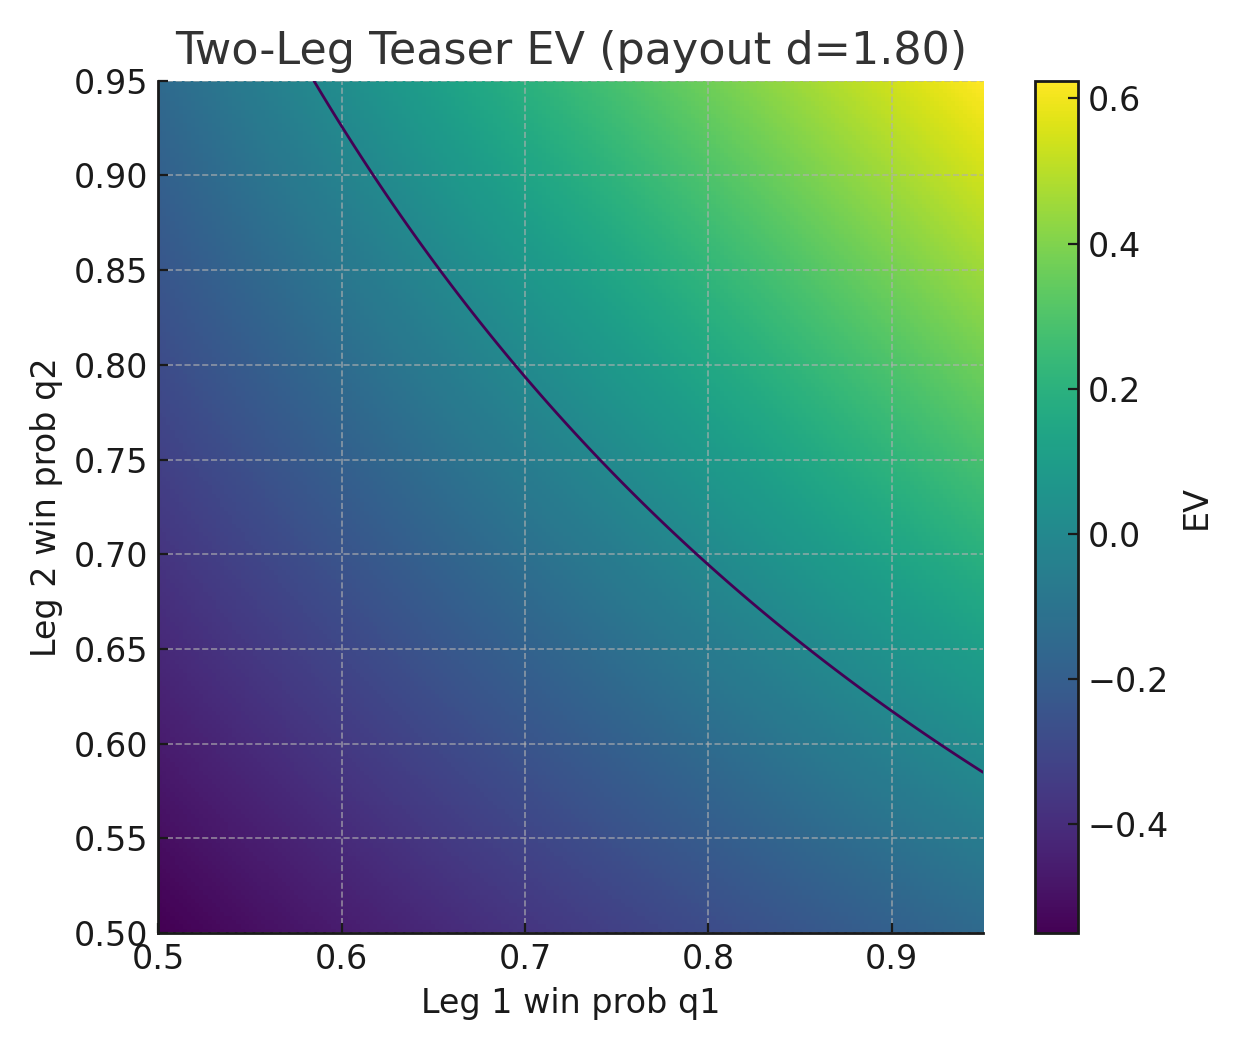
\includegraphics[width=0.85\textwidth]{analysis/figures/out/teaser_ev_heatmap.pdf}
  \caption{Teaser EV heatmap grid across legs and prices.}
  \label{fig:teaser-ev-heatmap}
\end{figure}
\end{verbatim}

\subsection{Bankroll Trajectory (Monte Carlo)}
\paragraph{Purpose.} Visualize bankroll distribution under fractional Kelly.
\paragraph{Outputs.} \texttt{bankroll\_ensemble.pdf}.
\paragraph{LaTeX.}
\begin{verbatim}
\begin{figure}[t]
  \centering
  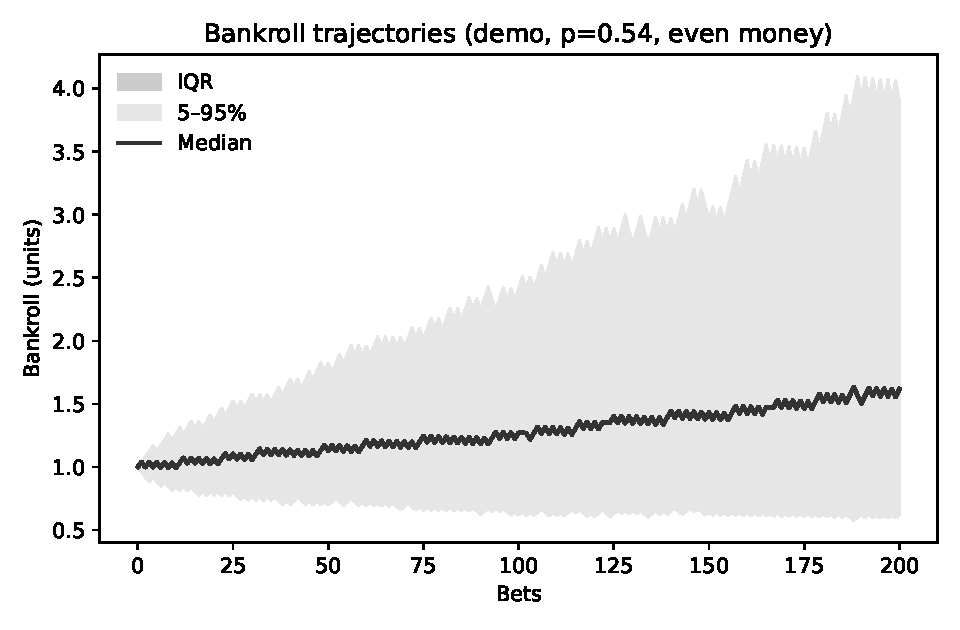
\includegraphics[width=0.62\textwidth]{analysis/figures/out/bankroll_ensemble.pdf}
  \caption{Simulated bankroll trajectories (1{,}000 paths) under 0.5-Kelly.
           Dark band: interquartile range; light band: 5--95\% envelope.}
  \label{fig:bankroll-ensemble}
\end{figure}
\end{verbatim}

\subsection{File Naming \& Captions}
\begin{itemize}
  \item Use kebab- or snake-case names; include season/week where relevant.
  \item Captions are descriptive, sentence case, and stand-alone (explain axes/units).
  \item Labels: \verb|\label{fig:<topic>-<variant>}| for deterministic cross-referencing.
\end{itemize}

\section{Placement Heuristics}
\begin{itemize}
  \item Use margin sparklines for small supporting trends (CLV, weekly error).
  \item Use inline figures for primary results (calibration, EV curves).
  \item Push large grids/heatmaps to the appendix; cross-reference from main text.
\end{itemize}
